\chapter{音声合成と音声認識}
\section{音声合成}
音声合成とは何でしょう。それは、人間の声を人工的に機械で作り出すことです。みなさんが目にするもので言えば、例えばソフトバンクが制作するpepper(図\ref{pepper})というロボットがあります。

\begin{figure}[H]
\begin{center}
    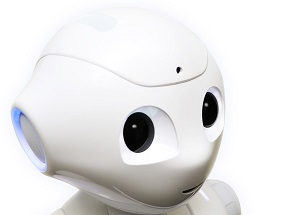
\includegraphics[width=0.5\linewidth]{images/chap06/text06-img001.jpg}
    \caption{pepper (softbank)}
    \label{pepper}
\end{center}
\end{figure}

これは声を出して利用者とコミュニケーションを取ります。pepperから声が出るのは、中に人間が入っているわけではありません。読み上げたい文章があったとき、それにマッチした音声を生成し、スピーカーから発しているのです。
今回は音声を合成するために、OpenJTalkと呼ばれる音声合成のためのソフトウェアを使います。OpenJTalkは、読み上げたい文章と、ひらがなごとの音(厳密にはもう少し多種の音)を入力し、対応する音声ファイルを出力します(図\ref{OpenJTalkの入出力})。

\begin{figure}[H]
\begin{center}
    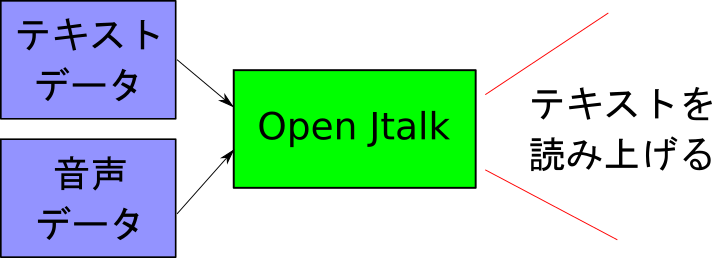
\includegraphics[width=\linewidth]{images/chap06/text06-img011.png}
    \caption{OpenJTalkの入出力}
    \label{OpenJTalkの入出力}
\end{center}
\end{figure}

\begin{tcolorbox}[title=\useOmetoi]
\begin{enumerate}
\item 音声合成とはなんですか。20字以内で説明してください。\\
\underline{答え.\hspace{0.8\linewidth}}
\item 音声合成をするにはパソコンに何を準備する必要がありますか。3つ挙げてください。\\
\underline{答え.\hspace{0.8\linewidth}}
\end{enumerate}
\end{tcolorbox}